\section{Historia i rozwój robotyki}
Robotyka jest stosunkowo młodą dziedziną nauki łączącą różne gałęzie nauk
technicznych i nie tylko. Do pełnego zrozumienia zagadnień współczesnej robotyki
oraz budowy i zastosowań robotów konieczna jest niejednokrotnie rozległa wiedza
na temat elektroniki, mechaniki, inżynierii przemysłowej, matematyki oraz
szeroko pojętej informatyki. Ponadto wiele nowopowstałych gałęzi wiedzy
zajmujących się rozwojem sztucznej inteligencji, modelowaniem sztucznego życia czy rozwojem
inżynierii wiedzy coraz częściej staje się nierozerwalnie związane z problemami
współczesnej robotyki. Nie należy zapominać również o tym, że rozwój inżynierii
wytwarzania oraz automatyki przemysłowej pozwala na nieustanny rozwój robotyki z
którą mamy do czynienia w przemyśle w dniu dzisiejszym.\\
\\
Pojęcie ``Robot'' w literaturze pojawił się po raz pierwszy w sztuce czeskiego
pisarza Karel'a Capka w roku 1920. Termin ``robot'' oznacza w języku czeskim
pracę lub służbę przymusową. Nieco ponad 20 lat później, amerykański uczony i
pisarz Isaac Assimov w jednym ze swoich opowiadań po raz pierwszy używa słowa
robotyka. W kolejnych latach Assimov w swojej twórczości niejednokrotnie wraca
do problemu robotyki skutkiem czego jest wydanie w 1950 roku zbioru opowiadań
pod tytułem ``Ja, robot''. Jako ciekawostkę można dodać, że w wydanym w 1942
roku opowiadaniu pod tytułem ``Zabawa w berka'', Assimove wprowadza trzy prawa
robotyki, według których zdaniem autora powinny być programowane roboty.
\begin{description}
\item[Prawo pierwsze] \hfill \\
Robot nie może zranić istoty ludzkiej, ani przez zaniedbanie narazić człowieka
na zranienie. 
\item[Prawo drugie] \hfill \\
Robot musi spełniać polecenia wydawane przez człowieka, poza poleceniami
sprzecznymi z prawem pierwszym.
\item[Prawo trzecie] \hfill \\
Robot musi chronić samego siebie dopóki nie jest to sprzeczne z prawami
pierwszym i drugim.
\end{description} 
Nieco później, Isaac Assimov, jako uzupełnienie i prawo nadrzędne dodaje prawo
zerowe o następującym brzmieniu ``Robot nie może szkodzić ludzkości, ani przez zaniedbanie narazić ludzkości na
szkodę''. Oprócz wspomnianych powyżej podstawowych praw, zdefiniowano również
inne prawa wynikające z prowadzonych badań w tej dziedzinie i rozwoju robotyki.\\
\\
Dzięki gwałtownemu rozwojowi techniki w czasie II wojny światowej w roku 1956
GC. Devol i JF. Engelberger zainspirowani twórczością Assimov'a zaprojektowali i
stworzyli pierwszy w dziejach ludzkości działający egzemplarz robota.
Engelberger założył firmę pod nazwą ``Unimation'' zajmującą się automatyzacją,
pierwszym robotem stworzonym przez firmę Engelbergera był robot nazwany
``Unimate''. Został on zainstalowany w fabryce General Motors w Trenton gdzie
został przystosowany do obsługi wysokociśnieniowej maszyny odlewniczej. W
kolejnych latach roboty firmy ``Unimation'' znalazły swoje zastosowanie w innych
gałęziach przemysłu, a sam Engelberger otrzymał miano ojca robotyki.\\
\\
Nieco później, bo w roku 1979 Robotics Industries Association 
zdefiniowało robota jako wielofunkcyjny, programowalny manipulator
zaprojektowany do przenoszenia materiałów, narzędzi, części urządzeń poprzez
serię programowalnych ruchów wykonywanych w celu realizacji różnych zadań.
W myśl wspomnianej definicji jedną z podstawowych cech robota jest jego
progrmowalność i możliwość dostosowywania się do zmiennych warunków środowiska
pracy. \\
Pierwsze roboty projektowano z myślą o zastosowaniu ich do realizacji
elementarnych zadań związanych z przenoszeniem elementów z jednego punktu do
drugiego. Program pracy robota miał więc charakter sekewencji operacji
prowadzących do realizacji określonego przez programistę zadania. W miarę
rozwoju technicznego, stawiane przed robotami zadania wymusiły użycie przez
konstruktorów czujników które pozwalały na zwiększenie poziomu interakcji
robotów z otoczeniem, a co za tym idzie umożliwiły realizowanie zadań o wysokim
stopniu złożoności. Od tego momentu kierunek rozwoju robotyki obrał
sobie za cel stworzenie maszyny na tyle uniwersalnej i niezależnej aby mogła
nosić miano androida. Jednak do realizacji tego zadania konieczne jest
opracowanie sztucznej inteligencji na którą z pewnością przyjdzie nam jeszcze
trochę poczekać. \\
\\
Pierwszym krokiem na drodze do stworzenia androida było oderwanie robota od
stałego miejsca instalacji i pozwolenie mu w miarę możliwości swobodne
poruszanie się dostępnej mu przestrzeni roboczej. Tak powstała klasa robotów
które mogą przemieszczać się za pomocą kół, gąsienic czy nawet kończyn lub
odnóży. Roboty tego typu potrafią pływać, latać i sprawnie poruszać się
po lądzie dodatkowym ich atutem jest fakt iż większość z nich posiada niemal
całkowitą autonomię i ograniczona jest jedynie poprzez wielkość otoczenia w
jakim zostały umieszczone. Takim sposobem roboty powstała grupa robotów
nazywanych robotami mobilnymi. Cechą wspólną wszystkich urządzeń z tej rodziny
była umiejętność swobodnego przemieszczania się oraz analiza najbliższego
otoczenia. Na tej podstawie maszyna mogła przeprowadzić wnioskowanie pozwalające
na podejmowanie dalszych akcji czy też zakomunikowanie użytkownikowi odczytanych
parametrów środowiska.\newpage
Historię robotów mobilny zapoczątkował amerykański Uniwersytet w Stanford gdyż
w roku 1968 jako pierwszy stworzył w pełni działający model robota mobilnego pod
nazwą Shakey. Nazwa została zainspirowana szarpanymi ruchami z jakimi robot się
poruszał. Głównym zadaniem robota było modelowanie otoczenia w którym się
znajdował. W ślad za Uniwersytetem w Stanford ruszyło MIT. W roku 1983 posiadali
już pierwszy działający model robota swobodnie skaczącego. Niecałe 6
lat później MIT stworzyło pierwszego robota kroczącego wzorowanego na owadach.
Robot ten sterowany był za pomocą wielowarstwowych automatów o stanach
skończonych, a ze światem zewnętrznym komunikował się za pomocą czułek,
inklinometrów, czujników zbliżeniowych na podczerwień. Genghis, bo tak
nazwany został robot, posiadał na pokładzie 4 ośmiobitowe jednostki obliczeniowe, ważył
niecały kilogram i miał 35 cm długości.

\begin{figure}[hb]
 \centering
 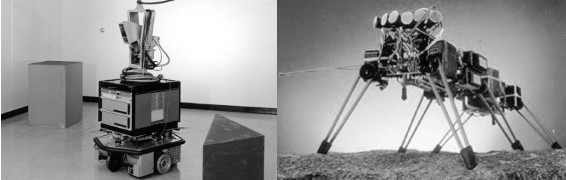
\includegraphics[height=50mm]{../images/ch01/shakey_and_genghis.png}
 \caption{Od lewej: Shakey (Stanford), Genghis (MIT) }
 \label{fig:RobotsHistory_Shakey_Genghis}
\end{figure}

Po sukcesie wspomnianych projektów,
rozwój robotów mobilnych następował już bardzo dynamiczne. W latach 90
powstawało wiele różnych modeli robotów o bardzo różnorodnych rodzajach napędów
oraz zestawach czujników umożliwiających interakcje ze światem zewnętrznym.

\begin{figure}[hb]
 \centering
 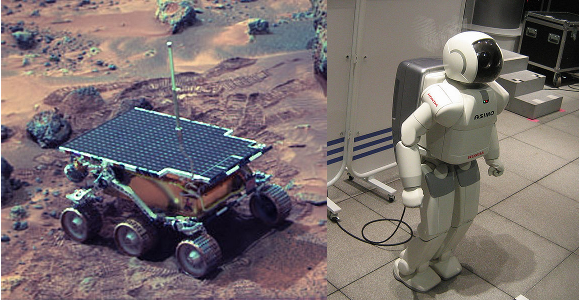
\includegraphics[height=60mm]{../images/ch01/pathfinder_and_asimo.png}
 \caption{Kolejno: Pathfinder (NASA), Asimo (Honda)}
 \label{fig:RobotsHistory_Pathfinder_Asimo}
\end{figure}

Swoistym ukoronowaniem prac było w 1997 roku stworzenie przez NASA robota o
nazwie Pathfinder. Robot wyposażony był w czujniki laserowe, stereowizję,
żyroskopy i inne rodzaje czujników o charakterze badawczym. Zasilany był on
bateriami słonecznymi które pozwoliły mu na 83 dni nieprzerwanej pracy podczas
której robot przebyło około 100 metrów i wykonał 230 manewrów. W ostatnich
latach do największych osiągnięć robotyki mobilnej można z pewnością zaliczyć
powstanie robotów humanoidalnych takich jak japoński ASIMO. Robot ten ważył 54
kg i posiadał 130 cm wysokości. Wersja z roku 2005 potrafiła biegnąc osiągnąć
prędkość dochodzącą nawet do do 6 km/h. Ponad to robot potrafił wchodzić w
interakcję z otoczającymi go ludźmi i przedmiotami. Urządzenie stworzone przez
inżynierów z firmy Honda potrafiło rozpoznawać gesty takie jak podanie ręki,
wskazanie kierunku czy machanie ręką na porzegnanie. Robot równie dobrze radził
sobie z rozpoznawaniem twarzy, dźwięków i analizą otaczającego go środowiska.
Potrafił on rozpoznać i omijać niebezpieczeństwa postawione na jego drodze jak
na przykład schody czy osoby poruszające się w jego kierunku.\\
\\
Obserwując postęp w dziedzinie robotyki można odnieść wrażenie iż w dzisiejszych
czasach roboty znalazły dla siebie zastosowanie niemal w każdej dziedzinie
życia. Od wielu lat sprawdzają się już w przemyśle, transporcie, budownictwie
oraz są niezastąpione w środowiskach nieprzyjaznych człowiekowi, takich jak
podmorskie głębiny czy otchłań kosmosu. Obszar zastosowań robotów jest
tak szeroki iż wydawać się może, że jedynym czynnikiem ograniczającym rozwój
współczesnej robotyki są względy czysto ekonomiczne. Nie staje to jednak na
przeszkodzie do projektowania i tworzenia przez konstruktorów z całego świata
rozwiązań powoli przybliżających ludzkość do stworzenia w pełni samodzielnego
oraz inteligentnego androida.
